%%%%%%%%%%%%%%%%%%%%%%%%%%%%%%%%
% BAYESIAN MULTILEVEL MODELING %
%%%%%%%%%%%%%%%%%%%%%%%%%%%%%%%%
Due to the lack of a unified terminology, we define a \textit{hierarchical} or \textit{multilevel model} as
``an overall system model that is hierarchically composed of deterministic and stochastic submodels''.
% SECTION OUTLINE
Important types of submodels comprise physical models of the deterministic system components (\cref{sec:PEM:Multilevel:ForwardModel}),
prior descriptions of parameter uncertainty and variability (\cref{sec:PEM:Multilevel:Uncertainty})
and residual representations of forward model prediction errors (\cref{sec:PEM:Multilevel:Residual}).
% GENERIC MODEL
From these submodels we will assemble a generic Bayesian multilevel model (\cref{sec:PEM:Multilevel:Overall}).
This will represent the overall system under consideration including its deterministic and probabilistic aspects.

\subsection{Forward model: Deterministic subsystem} \label{sec:PEM:Multilevel:ForwardModel}
% FORWARD MODEL: PHYSICS
A so-called \textit{forward model} is a mathematical representation of the physical system or phenomenon under investigation.
More formally the forward model is a function
\begin{equation} \label{eq:PEM:Multilevel:ForwardModel}
  \begin{aligned}
    \mathcal{M} \colon \mathcal{D}_{\bm{m}} \times \mathcal{D}_{\bm{x}} \times \mathcal{D}_{\bm{\zeta}} \times \mathcal{D}_{\bm{d}} &\rightarrow \mathcal{D}_{\perfect{\bm{y}}}\\
    (\bm{m},\bm{x},\bm{\zeta},\bm{d}) &\mapsto \perfect{\bm{y}} = \mathcal{M}(\bm{m},\bm{x},\bm{\zeta},\bm{d}),
  \end{aligned}
\end{equation}
that maps inputs \((\bm{m},\bm{x},\bm{\zeta},\bm{d}) \in \mathcal{D}_{\bm{m}} \times \mathcal{D}_{\bm{x}} \times \mathcal{D}_{\bm{\zeta}} \times \mathcal{D}_{\bm{d}}\)
from its domain to outputs \(\perfect{\bm{y}} \in \mathcal{D}_{\perfect{\bm{y}}}\) from its codomain.
% PARAMETERS / PREDICTIONS
Forward model arguments \((\bm{m},\bm{x},\bm{\zeta},\bm{d})\) constitute physical parameters, while its responses \(\perfect{\bm{y}}\) are predictions of observable quantities.
\par % FORWARD MODEL INPUTS
We distinguish between four different types of forward model inputs.
They differ in their (un)certain nature when a number of experiments is carried out.
There are fixed albeit unknown model parameters \(\bm{m} \in \mathcal{D}_{\bm{m}}\) that are subject to epistemic uncertainty,
two different types of inputs \(\bm{x} \in \mathcal{D}_{\bm{x}}\) and \(\bm{\zeta} \in \mathcal{D}_{\bm{\zeta}}\) that are subject to aleatory variability
and well-known experimental conditions \(\bm{d} \in \mathcal{D}_{\bm{d}}\).

\subsection{Prior model: Input uncertainty} \label{sec:PEM:Multilevel:Uncertainty}
%%%%%%%%%%%%%%%%%%%%%%%%%%%
% EXPERIMENTAL CONDITIONS %
%%%%%%%%%%%%%%%%%%%%%%%%%%%
Forward model inputs \(\bm{d}\) constitute perfectly known conditions that prevail during experimentation.
In line with this they are deterministic arguments of the forward model.
Experimental conditions may differ throughout the experiments, i.e.\ each of the experiments \(i=1,\ldots,n\) is conducted being subject to an experiment-specific condition \(\bm{d}_i\).
%%%%%%%%%%%%%%%%%%%%%%%%
\par % MODEL PARAMETER %
%%%%%%%%%%%%%%%%%%%%%%%%
Proper forward model parameters \(\bm{m}\) are constant throughout the experiments \(i=1,\ldots,n\), yet they have unknown values.
In Bayesian fashion the available prior or expert knowledge about the true parameter values is represented as a random variable or vector
\begin{equation} \label{eq:PEM:Multilevel:ParametricPriorM}
  \bm{M} \sim \pi_{\bm{M}} (\bm{m}).
\end{equation}
The Bayesian prior distribution \(\pi_{\bm{M}} (\bm{m})\) quantifies a subjective degree of plausibility or belief about the true parameter values \(\bm{m}\).
This is the Bayesian account for \textit{epistemic uncertainty}.
% REDUCIBILITY
The uncertainty is reducible in the sense that Bayesian data analysis gives rise to a posterior probability model.
%%%%%%%%%%%%%%%%%%%%%%%%%%
\par % KNOWN VARIABILITY %
%%%%%%%%%%%%%%%%%%%%%%%%%%
Forward model inputs \(\bm{\zeta}\) are subject to a form of variability that is well-known, e.g.\ it could be ascertained in previous experiments or due to prior considerations.
Rather than being constant throughout the experiments \(i=1,\ldots,n\), these variable inputs take on experiment-specific realizations \(\bm{\zeta}_i\), all of which are unknown.
The corresponding Bayesian prior representation is as mutually independent random variables
\begin{equation} \label{eq:PEM:Multilevel:StructuralPriorZ}
  \bm{Z}_i \sim f_{\bm{Z}}(\bm{\zeta}_i \distparam \bm{\theta}_{\bm{Z}_i}), \;\, \text{for} \;\, i=1,\ldots,n.
\end{equation}
Distributions \(f_{\bm{Z}}(\bm{\zeta}_i \distparam \bm{\theta}_{\bm{Z}_i})\) specify prior knowledge about the experiment-specific unknowns that is of structural quality.
They are prescribed by well-known hyperparameters \(\bm{\theta}_{\bm{Z}_i} \in \mathcal{D}_{\bm{\theta}_{\bm{Z}}}\), e.g.\ shape, scale and dependency parameters, that possibly differ across the experiments.
Due to stochastic independence, the appropriate joint Bayesian prior model follows as
\begin{equation} \label{eq:PEM:Multilevel:JointStructuralPriorZ}
  (\bm{Z}_1,\ldots,\bm{Z}_n) \sim \prod\limits_{i=1}^n f_{\bm{Z}}(\bm{\zeta}_i \distparam \bm{\theta}_{\bm{Z}_i}).
\end{equation}
This is a Bayesian conception of \textit{aleatory variability}, i.e.\ an uncertainty that is of structural nature.
Hereinafter this probability model will also be referred to as \textit{prescribed uncertainty}.
% IRREDUCIBILITY
It is irreducible in the sense that by Bayesian data analysis of the experiments \(i=1,\ldots,n\) ``past'' realizations \(\bm{\zeta}_i\) can be inferred in principle,
whereas the knowledge about ``future'' realizations \(\bm{\zeta}_{\further{i}}\) in further experiments \(\further{i} = n+1,\ldots,n+\further{n}\) cannot be improved.
``Future'' realizations still feature a structural uncertainty \(\bm{Z}_{\further{i}} \sim f_{\bm{Z}}(\bm{\zeta}_{\further{i}} \distparam \bm{\theta}_{\bm{Z}_{\further{i}}})\)
that is prescribed by hyperparameters \(\bm{\theta}_{\bm{Z}_{\further{i}}} \in \mathcal{D}_{\bm{\theta}_{\bm{Z}}}\).
%%%%%%%%%%%%%%%%%%%%%%%%%%%%
\par % UNKNOWN VARIABILITY %
%%%%%%%%%%%%%%%%%%%%%%%%%%%%
Another Bayesian notion of a similar type allows to account for forward model inputs \(\bm{x}\) that are subject to a sort of variability which itself is unknown.
For \(1=1,\ldots,n\) these variables take on experiment-specific realizations \(\bm{x}_i\), neither of which are known.
Bayesian prior modeling is build upon conditionally independent random variables
\begin{equation} \label{eq:PEM:Multilevel:StructuralPriorX}
  (\bm{X}_i \cond \bm{\Theta}_{\bm{X}}=\bm{\theta}_{\bm{X}}) \sim f_{\bm{X} \cond \bm{\Theta}_{\bm{X}}} (\bm{x}_i \cond \bm{\theta}_{\bm{X}}), \;\, \text{for} \;\, i=1,\ldots,n.
\end{equation}
The conditional probability distribution \(f_{\bm{X} \cond \bm{\Theta}_{\bm{X}}} (\bm{x}_i \cond \bm{\theta}_{\bm{X}})\) represents a structural kind of prior knowledge about the experiment-specific unknowns.
% HYPERPARAMETER
Its determining hyperparameters \(\bm{\theta}_{\bm{X}} \in \mathcal{D}_{\bm{\theta}_{\bm{X}}}\), e.g.\ location, dispersion and correlation parameters, themselves are fixed yet unknown.
Hence these hyperparameters are priorly modeled as a random vector
\begin{equation} \label{eq:PEM:Multilevel:ParametricPriorThetaX}
  \bm{\Theta}_{\bm{X}} \sim \pi_{\bm{\Theta}_{\bm{X}}} (\bm{\theta}_{\bm{X}}).
\end{equation}
The Bayesian prior distribution \(\pi_{\bm{\Theta}_{\bm{X}}} (\bm{\theta}_{\bm{X}})\) constitutes the subjective prior belief or available prior knowledge about the true hyperparameter values.
% PRIOR ELICITATION
In the statistical literature hyperprior elicitation is exhaustively discussed especially for variance hyperparameters \cite{Multilevel:Berger1996,Multilevel:Berger2005,Multilevel:Gelman2006:b}.
% EXCHANGEABILITY
Consequently the joint distribution of the unknowns of this prior model is given as
\begin{equation} \label{eq:PEM:Multilevel:JointStructuralPriorX}
  (\bm{X}_1,\ldots,\bm{X}_n,\bm{\Theta}_{\bm{X}}) \sim \left( \prod_{i=1}^n f_{\bm{X} \cond \bm{\Theta}_{\bm{X}}} (\bm{x}_i \cond \bm{\theta}_{\bm{X}}) \right) \pi_{\bm{\Theta}_{\bm{X}}} (\bm{\theta}_{\bm{X}}).
\end{equation}
The joint prior distribution of experiment-specific realizations follows by marginalizing \cref{eq:PEM:Multilevel:JointStructuralPriorX} over the hyperparameters \(\bm{\theta}_{\bm{X}}\).
Then one has
\begin{equation} \label{eq:PEM:Multilevel:Exchangeability}
  (\bm{X}_1,\ldots,\bm{X}_n) \sim \int\limits_{\mathcal{D}_{\bm{\theta}_{\bm{X}}}} \left( \prod\limits_{i=1}^n f_{\bm{X} \cond \bm{\Theta}_{\bm{X}}} (\bm{x}_i \cond \bm{\theta}_{\bm{X}}) \right)
  \pi_{\bm{\Theta}_{\bm{X}}} (\bm{\theta}_{\bm{X}}) \, \mathrm{d} \bm{\theta}_{\bm{X}}.
\end{equation}
This is a form of \textit{exchangeability} \cite{Multilevel:Draper1993,Multilevel:Bernardo1996} that realizes some ``similarity'' of the intermediate variables,
i.e.\ the joint distribution of the sequence \((\bm{X}_1,\ldots,\bm{X}_n)\) equals the one of \((\bm{X}_{\tau(1)},\ldots,\bm{X}_{\tau(n)})\) for any index permutation \(\tau \colon \{1,\ldots,n\} \rightarrow \{1,\ldots,n\}\).
In the present form \cref{eq:PEM:Multilevel:Exchangeability}, exchangeability establishes another Bayesian approach to aleatory variability.
% PARTIAL REDICUBILITY
Unlike the prescribed uncertainty in \cref{eq:PEM:Multilevel:JointStructuralPriorZ},  
this form of uncertainty is partially reducible in the sense that the ``fuzziness'' inherent in \cref{eq:PEM:Multilevel:Exchangeability} can be reduced by learning about \(\bm{\theta}_{\bm{X}}\) in ``past'' experiments \(i\).
``Past'' realizations \(\bm{x}_i\) can also be inferred, however, even if the hyperparameters \(\bm{\theta}_{\bm{X}}\) would be known, the realizations \(\bm{x}_{\further{i}}\) of ``future'' experiments \(\further{i}\)
would still carry the structural prior uncertainty \(\bm{X}_{\further{i}} \sim f_{\bm{X} \cond \bm{\Theta}_{\bm{X}}} (\bm{x}_{\further{i}} \cond \bm{\theta}_{\bm{X}})\).
%%%%%%%%%%%%%%%%%%%%%%
\par % SHORT SUMMARY %
%%%%%%%%%%%%%%%%%%%%%%
In short, on the one hand we have \textit{parametric priors} \(\pi_{\bm{M}} (\bm{m})\) and \(\pi_{\bm{\Theta}_{\bm{X}}} (\bm{\theta}_{\bm{X}})\)
that in \cref{eq:PEM:Multilevel:ParametricPriorM,eq:PEM:Multilevel:ParametricPriorThetaX} embody knowledge about global unknowns \(\bm{m}\) and \(\bm{\theta}_{\bm{X}}\).
On the other hand we have \textit{structural priors} \(f_{\bm{Z}}(\bm{\zeta}_i \distparam \bm{\theta}_{\bm{Z}_i})\) and
\(f_{\bm{X} \cond \bm{\Theta}_{\bm{X}}} (\bm{x}_i \cond \bm{\theta}_{\bm{X}})\) that encapsulate structural prior knowledge about the problem,
and that for \(i=1,\ldots,n\) establish the prior model of experiment-specific unknowns \(\bm{x}_i\) and \(\bm{\zeta}_i\) through \cref{eq:PEM:Multilevel:JointStructuralPriorZ,eq:PEM:Multilevel:Exchangeability}.

\subsection{Residual model: Output imperfection} \label{sec:PEM:Multilevel:Residual}
% RESIDUAL MODEL
Besides a representation of forward model input uncertainty and variability,
an integral constituent of statistical approaches to inversion is a \textit{residual representation} of forward model output discrepancy or imperfection.
Due to measurement errors, numerical approximations and general inadequacies, even if all inputs \((\bm{m},\bm{x}_i,\bm{\zeta}_i,\bm{d}_i)\) were perfectly known,
predictions \(\perfect{\bm{y}}_i = \mathcal{M}(\bm{m},\bm{x}_i,\bm{\zeta}_i,\bm{d}_i)\) are expected to deviate from real observations \(\bm{y}_i\).
These imperfections can be accounted for by a \textit{statistical data model}
\begin{equation} \label{eq:PEM:Multilevel:StatisticalDataModel}
  \bm{y}_i = \perfect{\bm{y}}_i + \bm{\varepsilon}_i = \mathcal{M}(\bm{m},\bm{x}_i,\bm{\zeta}_i,\bm{d}_i) + \bm{\varepsilon}_i,
  \;\, \text{for} \;\, i=1,\ldots,n,
\end{equation}
where residual terms \(\bm{\varepsilon}_i \in \mathcal{D}_{\bm{\varepsilon}}\) are assumed to be realizations of random variables \(\bm{E}_i \sim f_{\bm{E}}(\bm{\varepsilon}_i \distparam \bm{\Sigma}_i)\).
Commonly one employs normal distributions \(f_{\bm{E}}(\bm{\varepsilon}_i \distparam \bm{\Sigma}_i) = \mathcal{N}(\bm{\varepsilon}_i \distparam \bm{0},\bm{\Sigma}_i)\)
with mean \(\bm{0}\) and possibly experiment-specific, symmetric and positive-semidefinite covariance matrices \(\bm{\Sigma}_i\).
% RANDOM DATA
Consequently, through a change of variables whose Jacobian determinant equals one, observations are viewed as outcomes \(\bm{y}_i\) of random variables
\begin{equation} \label{eq:PEM:Multilevel:ResidualModel}
  (\bm{Y}_i \cond \bm{M} = \bm{m},\bm{X}_i = \bm{x}_i,\bm{Z}_i = \bm{\zeta}_i) \sim f_{\bm{E}} \big( \bm{y}_i-\mathcal{M}(\bm{m},\bm{x}_i,\bm{\zeta}_i,\bm{d}_i) \distparam \bm{\Sigma}_i \big),
  \;\, \text{for} \;\, i=1,\ldots,n.
\end{equation}
% CONDITIONAL STRUCTURE
For given values of the direct forward model inputs \((\bm{m},\bm{x}_i,\bm{\zeta}_i,\bm{d}_i)\),
data are viewed as random variables \((\bm{Y}_i \cond \bm{m},\bm{x}_i,\bm{\zeta}_i)\) with conditional distributions
\(f (\bm{y}_i \cond \bm{m},\bm{x}_i,\bm{\zeta}_i) = f_{\bm{E}} (\bm{y}_i-\mathcal{M}(\bm{m},\bm{x}_i,\bm{\zeta}_i,\bm{d}_i) \distparam \bm{\Sigma}_i)\).
Note that \(f (\bm{y}_i \cond \bm{m}, \allowbreak \bm{x}_i,\bm{\zeta}_i) = f (\bm{y}_i \cond \bm{m},\bm{x}_i,\bm{\zeta}_i,\bm{\theta}_{\bm{X}})\) is independent of \(\bm{\theta}_{\bm{X}}\).
\par % RESIDUAL CALIBRATION
The specification of the residual model, i.e.\ quantifying the parameters of \(\bm{\Sigma}_i\), is an essential part of calibrating the forward model and the experimental apparatus.
% PREDICTIVE ERROR CALIBRATION
In many experimental situations a model of the \textit{prediction error} is not known a priori, though.
Nevertheless, the structure of the prediction error model can be selected \cite{Bayesian:Simoen2013:a} and
its parameters can be introduced as unknown hyperparameters that undergo calibration \cite{Bayesian:Zhang2011}.
% SYSTEMATIC ERRORS & MODEL BIAS
This also includes systematic forward model deviations \cite{Bayesian:Kennedy2001,Bayesian:Arendt2012:a}.
% MODEL UNCERTAINTY
Moreover one could treat the form of the forward model \(\mathcal{M}\) itself as uncertain/random \cite{Bayesian:Droguett2008,Bayesian:Park2014}
and select the most plausible class via Bayesian model selection \cite{Bayesian:Beck2004,Bayesian:Yuen2010:b}.
% HIERARCHICAL MODELS
By adding another layer of uncertainty on top of the outlined setup and at a higher associated cost,
the aforementioned principles of assessing structural and parametric forward model uncertainty can be readily applied in multilevel models \cite{Bayesian:Draper1995}.
\par % ``PERFECT'' DATA
Based on random variable transformations, in \cref{sec:PEM:PerfectData} we will extend the framework by a model
for analyzing ``perfect'' observations \(\perfect{\bm{y}}_i = \mathcal{M}(\bm{m},\bm{x}_i,\bm{\zeta}_i,\bm{d}_i)\) in the zero-noise limit \(\lvert \bm{\varepsilon}_i \rvert \rightarrow 0\).
This mathematical formulation will explain the variability in the data exclusively by a Bayesian prior model of input variability as outlined in the preceding \cref{sec:PEM:Multilevel:Uncertainty}.

\subsection{Multilevel model: Overall system} \label{sec:PEM:Multilevel:Overall}
% (CONDITIONAL) INDEPENDENCE
We start from the premise that if not denoted or stated otherwise, random vectors and variables are (conditionally) independent,
e.g.\ the global forward model parameters \(\bm{M}\) and the hyperparameters \(\bm{\Theta}_{\bm{X}}\) are understood to be priorly independent.
Thus \(\pi(\bm{m},\bm{\theta}_{\bm{X}}) = \pi_{\bm{M}} (\bm{m}) \, \pi_{\bm{\Theta}_{\bm{X}}} (\bm{\theta}_{\bm{X}})\) applies for their joint prior distribution.
Note that this is not a necessity of the formulation, though.
% (CONDITIONAL) NOTATION
Moreover, we strictly reserve conditional notation for the stochastic dependency of random variables on outcomes of other random variables,
e.g.\ the aleatory variables \((\bm{X}_i \cond \bm{\theta}_{\bm{X}})\) are conditionally dependent on realizations \(\bm{\Theta}_{\bm{X}}=\bm{\theta}_{\bm{X}}\).
The stochastic variables \((\bm{Y}_i \cond \bm{m},\bm{x}_i,\bm{\zeta}_i)\) are conditioned on random outcomes \(\bm{M}=\bm{m}\), \(\bm{X}_i=\bm{x}_i\) and \(\bm{Z}_i=\bm{\zeta}_i\),
nonetheless they depend on deterministic quantities \(\bm{d}_i\) and \(\bm{\Sigma}_i\), too.
Similarly the aleatory variables \(\bm{Z}_i\) are dependent on \(\bm{\theta}_{\bm{Z}_i}\) in a way that is not explicitly indicated.
% BOOKKEEPING INDEX
In order to keep track of all stochastic and deterministic relations the index \(i\) serves as a bookkeeping mark.
\par % SUBMODELS
Deterministic aspects of the system are covered by the forward model \cref{eq:PEM:Multilevel:ForwardModel}.
Parametric priors in \cref{eq:PEM:Multilevel:ParametricPriorM,eq:PEM:Multilevel:ParametricPriorThetaX} and structural priors in
\cref{eq:PEM:Multilevel:StructuralPriorZ,eq:PEM:Multilevel:StructuralPriorX} represent input uncertainty and variability.
The model \cref{eq:PEM:Multilevel:ResidualModel} condenses basic assumptions regarding the prediction error.
% OVERALL MODEL
Altogether those submodels are combined into a greater model of the whole system.
The overall probability model is summarized as
\begin{subequations} \label{eq:PEM:Multilevel:Model}
  \begin{align}
    (\bm{Y}_i \cond \bm{m},\bm{x}_i,\bm{\zeta}_i) &\sim f_{\bm{E}} \big( \bm{y}_i-\mathcal{M}(\bm{m},\bm{x}_i,\bm{\zeta}_i,\bm{d}_i) \distparam \bm{\Sigma}_i \big), \label{eq:PEM:Multilevel:Model:Data}\\
    \bm{M} &\sim \pi_{\bm{M}} (\bm{m}), \label{eq:PEM:Multilevel:Model:ParametricPriorM}\\
    \bm{Z}_i &\sim f_{\bm{Z}}(\bm{\zeta}_i \distparam \bm{\theta}_{\bm{Z}_i}), \label{eq:PEM:Multilevel:Model:StructuralPriorZ}\\
    (\bm{X}_i \cond \bm{\theta}_{\bm{X}}) &\sim f_{\bm{X} \cond \bm{\Theta}_{\bm{X}}} (\bm{x}_i \cond \bm{\theta}_{\bm{X}}), \label{eq:PEM:Multilevel:Model:StructuralPriorX}\\
    \bm{\Theta}_{\bm{X}} &\sim \pi_{\bm{\Theta}_{\bm{X}}} (\bm{\theta}_{\bm{X}}). \label{eq:PEM:Multilevel:Model:ParametricPriorThetaX}
  \end{align}
\end{subequations}
% SUBJECTIVIST
Adopting a subjectivist viewpoint, this complex probability model \cref{eq:PEM:Multilevel:Model} formalizes degrees of belief of how the data have been realized in the experiments \(i=1,\ldots,n\).
% HIERARCHICAL STRUCTURE
According to our previous definition it is a generic Bayesian multilevel model.
% DAG
An intuitive representation of this multilevel model is provided by a directed acyclic graph (DAG) \cite{Bayesian:Koski2009,Bayesian:Kjaerulff2013} such as shown in \cref{fig:PEM:Multilevel:DAG}.
\begin{figure}[ht]
  \centering
  \includegraphics[height=6.5cm]{fig_PEM_DAG_Generic}
  \caption[DAG of the generic multilevel model]{DAG of the generic multilevel model.
           Vertices symbolize known (\(\vcenter{\hbox{\protect\includegraphics[height=1.2ex]{fig_Square}}}\))
           or unknown (\(\vcenter{\hbox{\protect\includegraphics[height=1.3ex]{fig_Circle}}}\)) quantities,
           while directed edges represent their deterministic (\(\vcenter{\hbox{\protect\includegraphics[height=1.0ex]{fig_Solid}}}\))
           or probabilistic (\(\vcenter{\hbox{\protect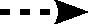
\includegraphics[height=1.0ex]{fig_Dashed}}}\)) relations.
           Global parameters \((\bm{m},\bm{\theta}_{\bm{X}})\) are subject to epistemic uncertainty,
           whereas experiment-specific realizations \((\tuple{\bm{x}_i},\tuple{\bm{\zeta}_i})\) are subject to aleatory variability.
           Known quantities comprise the data \(\tuple{\bm{y}_i}\) just as well as experiment-specific knowns
           \((\tuple{\bm{\theta}_{\bm{Z}_i}},\tuple{\bm{d}_i},\tuple{\bm{\Sigma}_i})\) located at different levels of the hierarchy.
          }
  \label{fig:PEM:Multilevel:DAG}
\end{figure}